\documentclass[aspectratio=169,11pt]{beamer}
% ============================================================
% PACKAGES
% ============================================================
\usepackage[utf8]{inputenc}
\usepackage{graphicx}
\usepackage{tikz}
\usetikzlibrary{positioning,calc}
\usepackage{xcolor}
\usepackage{amsmath}
\usepackage{amssymb}
\usepackage{listings}
\usepackage{array}
\usepackage{booktabs}
\usepackage{colortbl}
\usepackage{pifont}
\usepackage{hyperref}

% ============================================================
% COLOR SYSTEM
% ============================================================
\definecolor{primary}{RGB}{15,40,70}
\definecolor{secondary}{RGB}{25,92,124}
\definecolor{accent}{RGB}{41,197,180}
\definecolor{highlight}{RGB}{255,172,58}
\definecolor{light}{RGB}{239,245,249}
\definecolor{mid}{RGB}{220,228,235}
\definecolor{dark}{RGB}{31,35,40}
\definecolor{panel}{RGB}{247,250,252}
\definecolor{danger}{RGB}{185,65,65}

% ============================================================
% BEAMER THEME
% ============================================================
\usetheme{default}
\usecolortheme{default}

\setbeamercolor{normal text}{fg=dark,bg=white}
\setbeamercolor{structure}{fg=secondary}
\setbeamercolor{title}{fg=primary}
\setbeamercolor{subtitle}{fg=secondary}
\setbeamercolor{frametitle}{fg=white,bg=primary}

\setbeamercolor{block title}{bg=primary,fg=white}
\setbeamercolor{block body}{bg=panel,fg=dark}

\setbeamercolor{item projected}{bg=accent,fg=white}
\setbeamercolor{alerted text}{fg=highlight}
\setbeamercolor{example text}{fg=secondary}

\setbeamerfont{frametitle}{size=\Large,series=\bfseries}
\setbeamerfont{title}{size=\fontsize{30}{34}\selectfont,series=\bfseries}
\setbeamerfont{subtitle}{size=\large,series=\bfseries}

\setbeamertemplate{navigation symbols}{}

\setbeamertemplate{itemize item}
{\textcolor{accent}{\ding{108}}}

\setbeamertemplate{itemize subitem}
{\textcolor{secondary}{\ding{117}}}

\setlength{\itemsep}{0.25em plus 0.1em}
\setlength{\parsep}{0.15em}
\setlength{\topsep}{0.3em}

% ============================================================
% FRAME TITLE
% ============================================================
\setbeamertemplate{frametitle}{%
  \nointerlineskip
  \begin{beamercolorbox}[
      wd=\paperwidth,
      ht=2.7em,
      dp=0.6em,
      leftskip=0.8em,
      sep=0.25em
    ]{frametitle}
    \usebeamerfont{frametitle}\insertframetitle
  \end{beamercolorbox}
}

% ============================================================
% FOOTER
% ============================================================
\setbeamertemplate{footline}{%
  \leavevmode%
  \hbox{%
    \begin{beamercolorbox}[
        wd=.34\paperwidth,
        ht=2.5ex,
        dp=1ex,
        leftskip=1em
      ]{author in head/foot}
      \insertshortauthor
    \end{beamercolorbox}%
    \begin{beamercolorbox}[
        wd=.32\paperwidth,
        ht=2.5ex,
        dp=1ex,
        center
      ]{title in head/foot}
      \insertshorttitle
    \end{beamercolorbox}%
    \begin{beamercolorbox}[
        wd=.34\paperwidth,
        ht=2.5ex,
        dp=1ex,
        rightskip=1em,
        sep=0pt
      ]{date in head/foot}
      \insertframenumber{}/\inserttotalframenumber
    \end{beamercolorbox}%
  }%
  \vskip0pt%
}

\setbeamercolor{author in head/foot}{bg=secondary,fg=white}
\setbeamercolor{title in head/foot}{bg=primary,fg=white}
\setbeamercolor{date in head/foot}{bg=secondary,fg=white}

% ============================================================
% BACKGROUND
% ============================================================
\setbeamertemplate{background}{
  \begin{tikzpicture}[remember picture,overlay]
    \fill[light]
      (current page.south west)
      rectangle
      (current page.north east);

    \fill[secondary!10]
      (current page.north west)
      rectangle
      ([xshift=0.55\paperwidth,yshift=-0.18\paperheight]
       current page.north east);

    \fill[accent!18]
      ([xshift=0.73\paperwidth,yshift=-0.02\paperheight]
       current page.north west)
      rectangle
      ([xshift=\paperwidth,yshift=-0.22\paperheight]
       current page.north east);

    \draw[
      secondary!25,
      line width=0.4pt
    ]
      ([xshift=0.05\paperwidth,yshift=0.06\paperheight]
       current page.south west)
      grid[
        step=0.7cm
      ]
      ([xshift=-0.05\paperwidth,yshift=-0.06\paperheight]
       current page.north east);
  \end{tikzpicture}
}

% ============================================================
% CUSTOM COMMANDS
% ============================================================
\newcommand{\emphred}[1]{\textcolor{secondary}{#1}}
\newcommand{\emphhighlight}[1]{\textcolor{primary}{\textbf{#1}}}
\newcommand{\good}[1]{\textcolor{accent}{\textbf{#1}}}
\newcommand{\warning}[1]{\textcolor{highlight}{\textbf{#1}}}
\newcommand{\bad}[1]{\textcolor{danger}{\textbf{#1}}}

% ============================================================
% METADATA
% ============================================================
\title{SolSight}
\subtitle{
  \emphred{Solder Defect Detection System}
  --- Automatic Optical Inspection with AI
}
\author{AI-Powered Defect Detection}
\date{\today}

% ============================================================
% DOCUMENT
% ============================================================
\begin{document}

% ============================================================
% SLIDE 1 — TITLE
% ============================================================
\begin{frame}[plain]

\begin{tikzpicture}[remember picture,overlay]

    \fill[primary]
      (current page.north west)
      rectangle
      ([yshift=-2.9cm]current page.north east);

    \fill[accent]
      ([xshift=0.52\paperwidth,yshift=-0.8cm]
       current page.north west)
      rectangle
      ([xshift=0.84\paperwidth,yshift=-2.9cm]
       current page.north east);

    \fill[highlight!75]
      ([xshift=0.1\paperwidth,yshift=-1.6cm]
       current page.north west)
      rectangle
      ([xshift=0.35\paperwidth,yshift=-2.6cm]
       current page.north east);

\end{tikzpicture}

\vspace*{1.5cm}

\begin{center}

{\fontsize{30}{34}\selectfont
\bfseries\color{white}
SolSight}

\vspace{0.45cm}

{\large
\color{accent}
\textbf{Solder Defect Detection System}}

\vspace{0.7cm}

{\large
\color{white}
Unsupervised Anomaly Detection for PCB Assembly}

\vspace{0.8cm}

\begin{beamercolorbox}[
    wd=0.82\paperwidth,
    rounded=true,
    shadow=true,
    leftskip=1em,
    sep=0.7em
  ]{block body}

\begin{itemize}

    \item
    \emphhighlight{Fully convolutional autoencoder}
    for optical inspection

    \item
    \emphred{Resolution-flexible}
    anomaly detection

    \item
    \emphred{No labeled real-world defects}
    required for initial training

\end{itemize}

\end{beamercolorbox}

\end{center}

\end{frame}


% ============================================================
% SLIDE 2 — THE PROBLEM
% ============================================================
\begin{frame}\frametitle{\emphred{The Problem}}

\vspace{0.25cm}

\begin{center}

{\Large
\textbf{PCB inspection is still constrained by the data problem.}}

\end{center}

\vspace{0.5cm}

\begin{itemize}

    \item
    Manual solder-joint inspection is
    \emphred{slow and difficult to scale}.

    \item
    Defects are relatively rare compared with normal production.

    \item
    Supervised inspection systems require
    \emphred{representative labeled defect examples}.

    \item
    New boards, cameras, lenses, and manufacturing conditions
    introduce domain variation.

\end{itemize}

\vspace{0.6cm}

\begin{beamercolorbox}[
    wd=0.9\paperwidth,
    rounded=true,
    shadow=true,
    sep=0.8em
  ]{block body}

\begin{center}

\large
\textbf{
What if the system only needed to learn what a
good solder joint looks like?
}

\end{center}

\end{beamercolorbox}

\end{frame}


% ============================================================
% SLIDE 3 — THE CLAIM
% ============================================================
\begin{frame}\frametitle{\emphred{The Core Result}}

\begin{center}

{\fontsize{44}{48}\selectfont
\bfseries
\color{accent}
0.879}

\vspace{0.05cm}

{\normalsize
\bfseries
AUROC on real physical solder-joint data}

\vspace{0.3cm}

\begin{beamercolorbox}[
    wd=0.86\paperwidth,
    rounded=true,
    shadow=true,
    sep=0.5em
  ]{block body}

\begin{center}
\normalsize
\textbf{Trained entirely on synthetic renders.}

\vspace{0.08cm}

Tested \emphhighlight{zero-shot}
on real hardware it had never seen.

\vspace{0.08cm}

No labeled real-world defects were used for training.
\end{center}

\end{beamercolorbox}

\vspace{0.3cm}

{\footnotesize
The rest of this presentation answers three questions:
\textbf{Why does it work?}
\quad
\textbf{Does it generalize?}
\quad
\textbf{Where does it fail?}
}

\end{center}

\end{frame}


% ============================================================
% SLIDE 4 — HOW IT WORKS
% ============================================================
\begin{frame}\frametitle{\emphred{Insight: Learn Normal, Flag Reconstruction Failure}}

\begin{center}
\small
\textbf{A normal solder joint should reconstruct itself.
An abnormal one should leave a measurable reconstruction error.}
\end{center}

\vspace{0.15cm}

\begin{center}

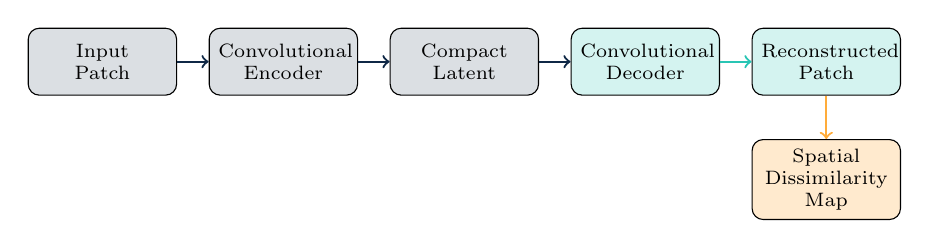
\begin{tikzpicture}[
    node distance=0.4cm,
    every node/.style={font=\scriptsize},
    box/.style={
        draw,
        rounded corners,
        minimum height=0.85cm,
        text width=1.65cm,
        align=center
    }
]

\node[
    box,
    fill=primary!15
] (input)
{Input\\Patch};

\node[
    box,
    fill=primary!15,
    right=of input
] (encoder)
{Convolutional\\Encoder};

\node[
    box,
    fill=primary!15,
    right=of encoder
] (latent)
{Compact\\Latent};

\node[
    box,
    fill=accent!20,
    right=of latent
] (decoder)
{Convolutional\\Decoder};

\node[
    box,
    fill=accent!20,
    right=of decoder
] (recon)
{Reconstructed\\Patch};

\node[
    box,
    fill=highlight!25,
    below=0.55cm of recon
] (score)
{Spatial\\Dissimilarity Map};

\draw[
    ->,
    thick,
    primary
]
(input) -- (encoder);

\draw[
    ->,
    thick,
    primary
]
(encoder) -- (latent);

\draw[
    ->,
    thick,
    primary
]
(latent) -- (decoder);

\draw[
    ->,
    thick,
    accent
]
(decoder) -- (recon);

\draw[
    ->,
    thick,
    highlight
]
(recon) -- (score);

\end{tikzpicture}

\end{center}

\vspace{0.15cm}

\begin{itemize}
    \item Training uses \emphred{normal solder-joint examples}
    rather than an exhaustive defect taxonomy.
    \item The model is fully convolutional:
    \emphred{no dense layers tie it to one input resolution}.
    \item A custom differentiable SSIM implementation produces a
    \emphred{spatial anomaly map}, rather than only one global score.
\end{itemize}

\end{frame}


% ============================================================
% SLIDE 5 — GENERALIZATION
% ============================================================
\begin{frame}\frametitle{\emphred{Generalization Beyond Training Resolution}}

\begin{center}
{\fontsize{32}{36}\selectfont
\bfseries
\color{accent}
0.862}

{\footnotesize AUROC at 32$\times$32 px}

\vspace{0.08cm}

\begin{beamercolorbox}[
    wd=0.84\paperwidth,
    rounded=true,
    shadow=true,
    sep=0.3em
  ]{block body}
\begin{center}
\footnotesize
\textbf{32 px was never used as a training tier.}
The model was trained on
\emphhighlight{16 px, 64 px and 128 px}
patches, yet achieved
\emphred{0.862 AUROC}
at the unseen 32 px resolution.
\end{center}
\end{beamercolorbox}

\vspace{0.1cm}

\footnotesize
\begin{tabular}{c|c|c}
\textbf{Resolution} & \textbf{Training Exposure} & \textbf{AUROC} \\
\hline
16 px & Trained & \good{0.940} \\
32 px & \warning{Zero-shot} & \good{0.862} \\
64 px & Trained & \good{0.963} \\
128 px & Trained & \good{0.850} \\
\end{tabular}

\vspace{0.08cm}

\scriptsize
Two independent forms of generalization now emerge:
\textbf{unseen resolution} and
\textbf{unseen physical hardware}.
\end{center}

\end{frame}


% ============================================================
% SLIDE 6 — FAILURE BOUNDARIES
% ============================================================
\begin{frame}\frametitle{\emphred{Where It Breaks --- And Why We Know}}

\begin{center}
\footnotesize\itshape
We did not only measure where the system works.
We deliberately mapped where it stops working.
\end{center}

\vspace{0.2cm}

\resizebox{0.98\textwidth}{!}{
\small
\begin{tabular}{|l|c|c|l|}
\hline
\textbf{Dimension} & \textbf{Observed Safe Range} & \textbf{Breaking Region} & \textbf{Observed Cause} \\
\hline
Spatial Resolution & $16$--$160$ px & $\leq 14$ px & SSIM window becomes too large \\
\hline
Defect Footprint & $\geq 1.5\%$ area & $<0.5\%$ & Global threshold becomes insensitive \\
\hline
Sensor Noise & $\sigma \leq 0.01$ & $\sigma \geq 0.02$ & SSIM contrast penalty \\
\hline
\end{tabular}
}

\vspace{0.3cm}

\begin{beamercolorbox}[
    wd=0.9\paperwidth,
    rounded=true,
    sep=0.45em
  ]{block body}
\footnotesize
\textbf{The important part is not that it fails.}
The important part is that the failure boundaries are
\emphhighlight{measurable and explainable}.
\end{beamercolorbox}

\vspace{0.2cm}

\begin{itemize}
    \item High-resolution bridging recall exposes a
    \emphred{threshold calibration problem}, not an unexplained model collapse.
    \item Per-tier threshold calibration provides a practical mitigation.
    \item Stress testing establishes operating margins before deployment.
\end{itemize}

\end{frame}


% ============================================================
% SLIDE 7 — REAL WORLD VALIDATION
% ============================================================
\begin{frame}\frametitle{\emphred{Real Hardware: Zero-Shot Domain Transfer}}

\begin{center}
\small
\textbf{Synthetic training $\rightarrow$ physical solder joints}
\end{center}

\vspace{0.1cm}

\begin{center}
\footnotesize
\begin{tabular}{|l|c|l|}
\hline
\textbf{Metric} & \textbf{Result} & \textbf{Context} \\
\hline
Real-World AUROC & \good{0.879} & Zero-shot synth $\rightarrow$ real \\
\hline
Normal-Joint FPR & \good{0.0\%} & Site-calibrated threshold \\
\hline
Overall Defect Recall & \good{48.5\%} & Site-calibrated threshold \\
\hline
Misaligned Component Recall & \good{72.0\%} & Site-calibrated threshold \\
\hline
Excessive Solder Recall & 46.0\% & Site-calibrated threshold \\
\hline
\end{tabular}
\end{center}

\vspace{0.12cm}

\begin{beamercolorbox}[
    wd=0.91\paperwidth,
    rounded=true,
    shadow=true,
    sep=0.3em
  ]{block body}
\scriptsize
\textbf{Threshold calibration matters.}
The synthetic global threshold is below the real normal-joint
baseline; applying it directly produces excess anomaly flags.
Deployment uses $T_{\mathrm{real}} = 0.2387$ calibrated on target hardware.
\end{beamercolorbox}

\vspace{0.08cm}

{\tiny
Validation dataset: SolDef\_AI, Fontana, Calabrese et al., CC BY 4.0.
}

\end{frame}


% ============================================================
% SLIDE 8 — DEPLOYMENT
% ============================================================
\begin{frame}\frametitle{\emphred{From Model to Factory Workflow}}

\begin{center}
\small
\textbf{The deployment requirement is calibration, not defect labeling.}
\end{center}

\vspace{0.2cm}

\begin{center}
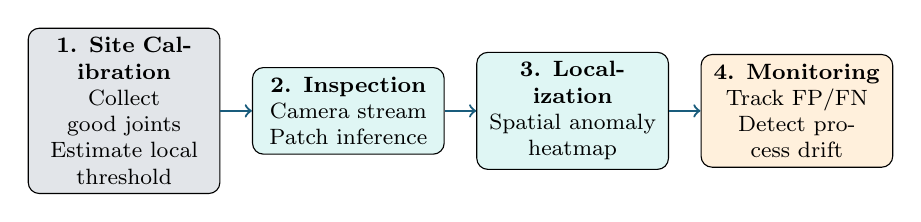
\begin{tikzpicture}[
    node distance=0.4cm,
    every node/.style={font=\footnotesize},
    process/.style={
        draw,
        rounded corners,
        fill=panel,
        minimum height=1.1cm,
        text width=2.2cm,
        align=center
    }
]
\node[process, fill=primary!12] (cal)
{\textbf{1. Site Calibration}\\
Collect good joints\\
Estimate local threshold};
\node[process, fill=accent!15, right=of cal] (inspect)
{\textbf{2. Inspection}\\
Camera stream\\
Patch inference};
\node[process, fill=accent!15, right=of inspect] (map)
{\textbf{3. Localization}\\
Spatial anomaly\\
heatmap};
\node[process, fill=highlight!18, right=of map] (monitor)
{\textbf{4. Monitoring}\\
Track FP/FN\\
Detect process drift};
\draw[->,thick,secondary] (cal) -- (inspect);
\draw[->,thick,secondary] (inspect) -- (map);
\draw[->,thick,secondary] (map) -- (monitor);
\end{tikzpicture}
\end{center}

\vspace{0.25cm}

\begin{itemize}
    \item Collect approximately
    \emphred{100--200 site-specific good samples}
    for threshold calibration.
    \item Generate anomaly scores in
    \emphred{real time ($<50$ ms per patch)}
    according to the current implementation.
    \item Expose the spatial DSSIM map so operators can inspect
    \emphred{where the anomaly is occurring}.
\end{itemize}

\end{frame}


% ============================================================
% SLIDE 9 — COMPARISON
% ============================================================
\begin{frame}\frametitle{\emphred{Where SolSight Fits}}

\resizebox{0.98\textwidth}{!}{
\small
\begin{tabular}{|l|c|c|c|}
\hline
\textbf{Capability} & \textbf{SolSight} & \textbf{Traditional AOI} & \textbf{Supervised DL} \\
\hline
Defect labels for initial training & \good{Not required} & Typically required & Typically required \\
\hline
Resolution flexibility & \good{Fully convolutional} & System-dependent & Architecture-dependent \\
\hline
Synthetic $\rightarrow$ real transfer & \good{0.879 AUROC} & N/A as learning claim & Requires validation / adaptation \\
\hline
Fine-grained defect localization & Spatial heatmap & Inspection-dependent & \good{Often strong} \\
\hline
Tooling maturity & Emerging & \good{Mature} & \good{Mature} \\
\hline
Labeling burden & \good{Low for initial training} & Depends on system & \bad{Potentially high} \\
\hline
\end{tabular}
}

\vspace{0.3cm}

\begin{beamercolorbox}[
    wd=0.9\paperwidth,
    rounded=true,
    sep=0.45em
  ]{block body}
\begin{center}
\footnotesize
\textbf{The differentiation is specific:}
\emphhighlight{low initial labeling burden
+ resolution flexibility
+ zero-shot synthetic-to-real validation}
\end{center}
\end{beamercolorbox}

\vspace{0.2cm}

\begin{center}
\footnotesize
Supervised approaches remain valuable where dense,
fine-grained localization and mature production tooling
are the primary requirements.
\end{center}

\end{frame}


% ============================================================
% SLIDE 10 — TECHNICAL IMPLEMENTATION
% ============================================================
\begin{frame}\frametitle{\emphred{Technical Foundation}}

\begin{itemize}
    \item \textbf{Language:} Python 3.10+
    \item \textbf{Deep Learning:} PyTorch 2.1+
    \item \textbf{Model:} Fully convolutional autoencoder
    \item \textbf{Similarity Metric:} Custom differentiable SSIM in PyTorch
    \item \textbf{Spatial Scoring:} Dynamic Gaussian windowing and spatial dissimilarity mapping
    \item \textbf{Evaluation:} ROC-AUC / AUROC, precision, recall and stress testing
\end{itemize}

\vspace{0.25cm}

\begin{center}
\small
\begin{tabular}{|l|c|}
\hline
\textbf{Artifact} & \textbf{Current Value} \\
\hline
Best checkpoint & \good{1.17 MB} \\
\hline
Maximum configured epochs & 30 \\
\hline
Configured batch size & 64 \\
\hline
Inference target & \good{$<$50 ms / patch} \\
\hline
\end{tabular}
\end{center}

\vspace{0.2cm}

\begin{center}
\footnotesize
Early stopping means the effective training duration can be
shorter than the configured 30-epoch maximum.
\end{center}

\end{frame}


% ============================================================
% SLIDE 11 — CURRENT DATA / EVIDENCE
% ============================================================
\begin{frame}\frametitle{\emphred{What We Can Reproduce Today}}

\begin{center}

{\normalsize
\textbf{The repository is part of the evidence.}}

\vspace{0.25cm}

\small
\begin{tabular}{|l|c|}
\hline
\textbf{Evidence} & \textbf{Current Repository State} \\
\hline
Synthetic patches & \good{2,100} \\
\hline
Best model checkpoint & \good{1.17 MB} \\
\hline
Real-world AUROC & \good{0.879} \\
\hline
Zero-shot 32 px AUROC & \good{0.862} \\
\hline
Site-calibrated real FPR & \good{0.0\%} \\
\hline
\end{tabular}

\vspace{0.3cm}

\begin{beamercolorbox}[
    wd=0.9\paperwidth,
    rounded=true,
    shadow=true,
    sep=0.45em
  ]{block body}
\begin{center}
\footnotesize
\textbf{Reproducibility principle}

The presentation reports the
\emphhighlight{current committed evaluation artifacts}
rather than numbers from an earlier experiment.
\end{center}
\end{beamercolorbox}

\vspace{0.2cm}

\footnotesize
Evaluation outputs include model metrics,
threshold configuration and stress-test summaries.

\end{center}

\end{frame}


% ============================================================
% SLIDE 12 — ROADMAP
% ============================================================
\begin{frame}\frametitle{\emphred{What Comes Next}}

\begin{itemize}

    \item
    \textbf{Edge Deployment}

    \begin{itemize}
        \item
        ONNX export and TVM-based optimization for
        ARM / FPGA targets.
    \end{itemize}

    \item
    \textbf{Multi-Modal Inspection}

    \begin{itemize}
        \item
        Combine visible and thermal imaging
        for additional defect evidence.
    \end{itemize}

    \item
    \textbf{Online Adaptation}

    \begin{itemize}
        \item
        Refine thresholds using controlled operator feedback
        and production statistics.
    \end{itemize}

    \item
    \textbf{Explainability}

    \begin{itemize}
        \item
        Develop richer defect-localization and
        importance visualization.
    \end{itemize}

\end{itemize}

\vspace{0.5cm}

\begin{beamercolorbox}[
    wd=0.9\paperwidth,
    rounded=true,
    sep=0.7em
  ]{block body}

\begin{center}

\textbf{
The immediate objective is not a larger model.
It is a more reliable operating envelope.
}

\end{center}

\end{beamercolorbox}

\end{frame}


% ============================================================
% SLIDE 13 — CLOSE
% ============================================================
\begin{frame}[plain]

\begin{center}

\vspace*{1.0cm}

{\fontsize{32}{36}\selectfont
\bfseries
\color{primary}
SolSight}

\vspace{0.45cm}

{\Large
\color{secondary}
\textbf{
Teaching inspection systems what ``normal'' looks like.
}}

\vspace{0.9cm}

\begin{beamercolorbox}[
    wd=0.78\paperwidth,
    rounded=true,
    shadow=true,
    sep=0.9em
  ]{block body}

\begin{center}

{\Large
\textbf{0.879 AUROC}
}

\vspace{0.15cm}

Zero-shot transfer from
\emphhighlight{synthetic training}
to
\emphhighlight{real solder-joint data}.

\end{center}

\end{beamercolorbox}

\vspace{1cm}

{\large
\textbf{Questions?}}

\vspace{0.55cm}

{\small
AI-Powered Optical Inspection
}

\end{center}

\end{frame}


% ============================================================
% SLIDE 14 — RESOURCES / CREDITS
% ============================================================
\begin{frame}\frametitle{\emphred{Resources \& Attribution}}

\begin{center}

\large
\textbf{\emphred{GitHub Repository}}

\vspace{0.2cm}

\href{https://github.com/stanmaluki/SolderDefectDetectionSystem}{
\texttt{github.com/stanmaluki/SolderDefectDetectionSystem}
}

\vspace{0.4cm}

\textbf{\emphred{Validation Dataset}}

\vspace{0.15cm}

SolDef\_AI \quad Fontana, Calabrese et al. \quad CC BY 4.0

\vspace{0.4cm}

\textbf{\emphred{Software}}

\vspace{0.15cm}

MIT License

\vspace{0.35cm}

{\footnotesize
Dataset attribution and licensing are retained explicitly
to distinguish project results from third-party validation data.
}

\end{center}

\end{frame}


% ============================================================
% END
% ============================================================
\end{document}
